\chapter{Prototyping Online Components}



\section{Section 1: The Role of APIs in IoT (Q7.1) [5M]}

\subsection{1. Definition}
An \textbf{API (Application Programming Interface)} is a set of defined rules, protocols, and tools that allows different software applications to communicate with each other. In IoT, APIs serve as the bridge between physical devices (sensors/actuators) and online services (cloud platforms, databases, third-party applications).


\subsection{2. Two Modes of API Usage in IoT}

\subsubsection{A. Consuming an Existing API}
\begin{itemize}
  \item   \textbf{Definition:} The IoT device or its gateway acts as a \textbf{client}, sending HTTP/REST requests to a third-party cloud API to retrieve or push data.
  \item   \textbf{Example:} A smart weather station sends a `GET` request to the OpenWeatherMap API to fetch a 5-day forecast, then displays it on a local e-paper screen.
  \item   \textbf{Key Benefit:} Eliminates the need to build your own data infrastructure; leverages existing, professionally maintained cloud services.
\end{itemize}

\subsubsection{B. Writing (Exposing) a New API}
\begin{itemize}
  \item   \textbf{Definition:} The IoT device or its edge gateway acts as a \textbf{server}, exposing its own RESTful API endpoints so that external applications can read sensor data or control actuators.
  \item   \textbf{Example:} A smart greenhouse exposes a REST API endpoint `GET /api/sensors/soil-moisture` that returns the latest soil moisture reading in JSON format. Any authorized mobile app or dashboard can query this endpoint.
  \item   \textbf{Key Benefit:} Makes the IoT device a first-class citizen of the web, enabling integration with any standard web client, automation platform, or other IoT devices.
\end{itemize}


\subsection{3. API Design Best Practices for IoT}
\begin{enumerate}
  \item \textbf{Use RESTful Conventions:} Map CRUD operations to HTTP verbs (`GET` = Read, `POST` = Create, `PUT` = Update, `DELETE` = Remove).
  \item \textbf{Use JSON for Data Payloads:} Lightweight, human-readable, and universally parsed by every programming language.
  \item \textbf{Implement Authentication:} Use API keys or OAuth 2.0 tokens to prevent unauthorized access to device endpoints.
  \item \textbf{Version the API:} Use URL-based versioning (e.g., `/api/v1/sensors/`) to allow backward-compatible upgrades.
\end{enumerate}


\section{Section 2: Cloud Computing in IoT and Smart Grid Applications (Q7.2) [10M]}

\subsection{1. Definition}
\textbf{Cloud Computing} in IoT refers to the use of remote, internet-hosted servers and services to store, process, and analyze the massive volumes of data generated by distributed IoT device networks. Instead of processing data locally on each constrained device, data is transmitted to powerful cloud data centers.


\subsection{2. Role of Cloud Computing in IoT}

\subsubsection{A. Data Storage}
\begin{itemize}
  \item   IoT devices generate continuous streams of time-stamped sensor readings. Cloud platforms provide virtually unlimited, elastically scalable storage (e.g., AWS S3, Google Cloud Storage, Azure Blob Storage) to archive this data.
\end{itemize}

\subsubsection{B. Data Processing and Analytics}
\begin{itemize}
  \item   Cloud servers run computationally intensive analytics pipelines (batch processing, stream processing, machine learning model training) that would be impossible on edge microcontrollers.
\end{itemize}

\subsubsection{C. Device Management}
\begin{itemize}
  \item   Cloud IoT platforms (e.g., AWS IoT Core, Azure IoT Hub, Google Cloud IoT) provide centralized dashboards for registering devices, monitoring their health, pushing Over-The-Air (OTA) firmware updates, and managing device twins (digital shadow copies).
\end{itemize}

\subsubsection{D. Application Hosting}
\begin{itemize}
  \item   Web dashboards, mobile app backends, and notification services are hosted in the cloud, providing users with real-time visibility into their IoT networks from anywhere in the world.
\end{itemize}


\subsection{3. Cloud Computing in Smart Grid Architecture}

\begin{figure}[H]
\centering
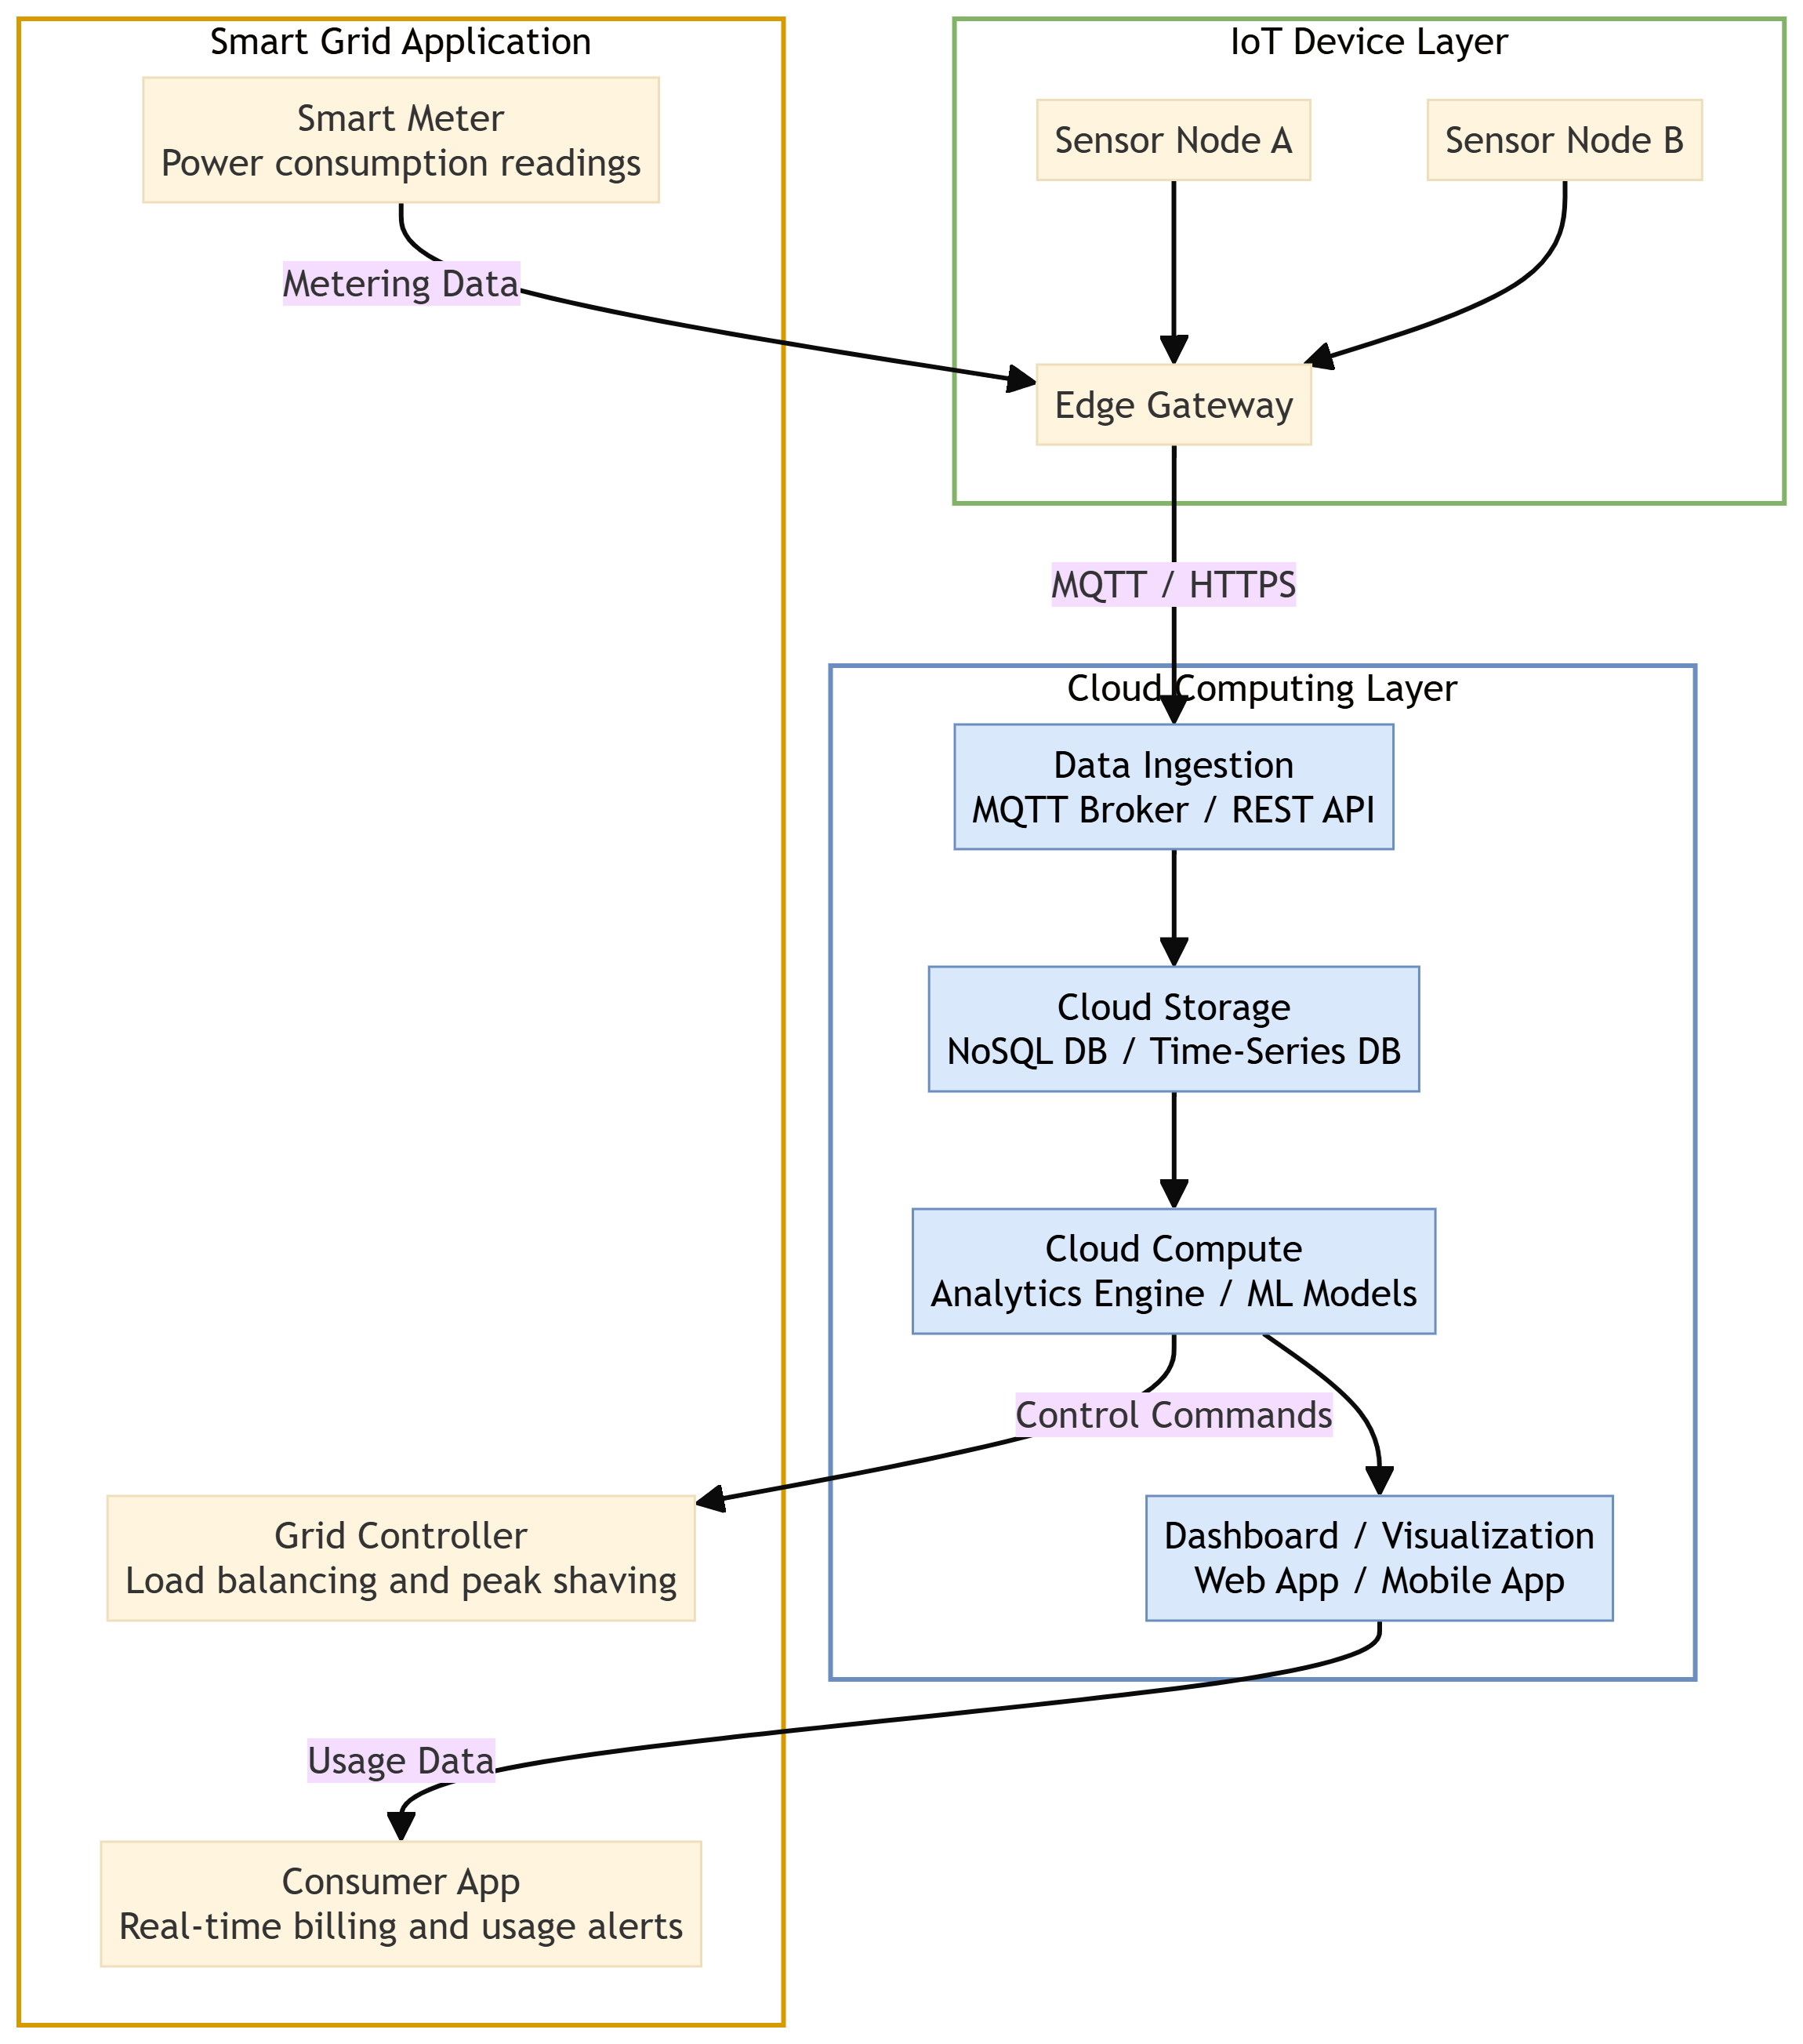
\includegraphics[width=0.75\textwidth,height=0.32\textheight,keepaspectratio]{../Images/chapter_07/cloud_iot_architecture.png}
\caption{Cloud IoT Architecture with Smart Grid Application}
\end{figure}

A \textbf{Smart Grid} is an electrical grid that uses IoT sensors, two-way digital communication, and cloud computing to monitor, analyze, and optimize the generation, distribution, and consumption of electricity.

\subsubsection{Key Components:}
\begin{enumerate}
  \item \textbf{Smart Meters:} Installed at consumer endpoints (homes, factories). They measure real-time electricity consumption and transmit readings to the cloud via cellular or Wi-Fi gateways.
  \item \textbf{Cloud Analytics Platform:} Receives metering data from millions of smart meters. Performs:
\end{enumerate}
\begin{itemize}
  \item   \textbf{Demand Forecasting:} Uses historical consumption patterns and weather data to predict future electricity demand.
  \item   \textbf{Load Balancing:} Dynamically reroutes power from over-supplied areas to under-supplied areas.
  \item   \textbf{Peak Shaving:} Identifies demand spikes and signals distributed battery storage systems to discharge, reducing strain on the central grid.
\end{itemize}
\begin{enumerate}
  \item \textbf{Consumer-Facing Applications:} Cloud-hosted dashboards and mobile apps allow consumers to view their real-time energy consumption, compare it against neighbors, and receive alerts when usage exceeds a threshold.
  \item \textbf{Grid Controller Integration:} The cloud sends automated control commands to grid substations and distributed energy resources (solar inverters, wind turbines) to adjust power output in real-time.
\end{enumerate}

\subsubsection{Advantages of Cloud in Smart Grid:}
\begin{enumerate}
  \item Centralized processing of millions of data points from distributed meters.
  \item Elastic scaling during peak demand periods.
  \item Historical trend analysis for long-term infrastructure planning.
\end{enumerate}

\subsubsection{Disadvantages:}
\begin{enumerate}
  \item \textbf{Latency:} Cloud round-trip delays may be too slow for mission-critical grid protection relay decisions.
  \item \textbf{Data Privacy:} Granular energy consumption patterns can reveal private behavioral details about households.
  \item \textbf{Connectivity Dependency:} A WAN or internet outage disconnects all meters from the analytics engine.
\end{enumerate}


\section{Section 3: Big Data Analytics in IoT (Q7.3) [10M]}

\subsection{1. Introduction}
IoT networks generate massive, high-velocity, heterogeneous data streams (sensor readings, log files, video frames, GPS coordinates). \textbf{Big Data Analytics} provides the methods and tools to extract actionable intelligence from this data deluge.


\subsection{2. The Four Levels of Data Analytics}

\begin{figure}[H]
\centering
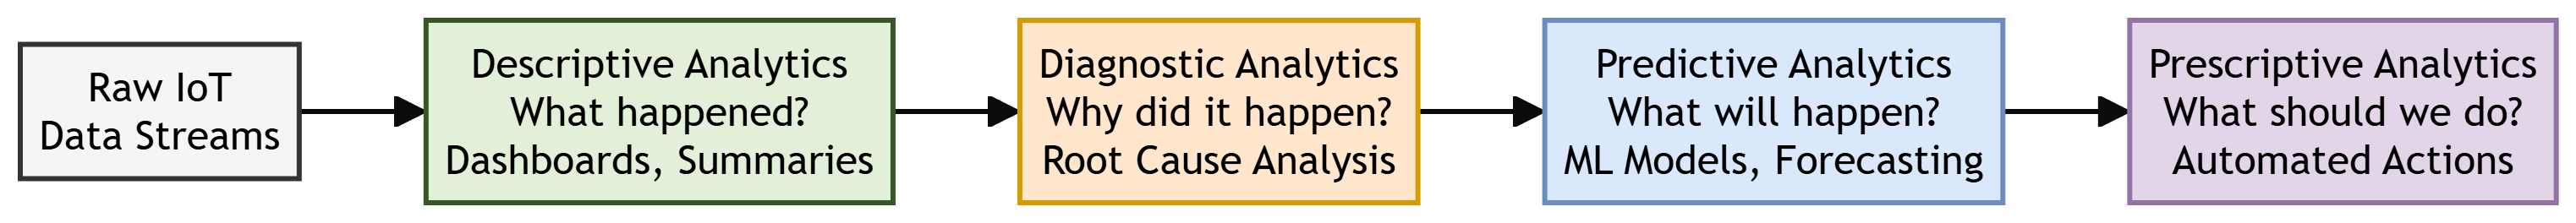
\includegraphics[width=0.75\textwidth,height=0.32\textheight,keepaspectratio]{../Images/chapter_07/big_data_analytics.png}
\caption{Big Data Analytics Pipeline for IoT}
\end{figure}

\subsubsection{Level 1: Descriptive Analytics ("What happened?")}
\begin{itemize}
  \item   \textbf{Objective:} Summarize raw historical data into understandable reports, charts, and dashboards.
  \item   \textbf{Techniques:} Aggregation, data visualization, statistical summaries (mean, median, min/max).
  \item   \textbf{IoT Use Case:} A factory floor dashboard displays the average temperature of 50 industrial ovens over the last 24 hours, flagging any that exceeded the safe threshold.
\end{itemize}

\subsubsection{Level 2: Diagnostic Analytics ("Why did it happen?")}
\begin{itemize}
  \item   \textbf{Objective:} Drill down into the data to identify the root cause of an observed event or anomaly.
  \item   \textbf{Techniques:} Correlation analysis, data mining, pattern detection, drill-down queries.
  \item   \textbf{IoT Use Case:} After a factory oven overheated, the system cross-references the oven's temperature logs with the coolant flow sensor logs and discovers that a coolant pump failed 30 minutes before the temperature spike.
\end{itemize}

\subsubsection{Level 3: Predictive Analytics ("What will happen?")}
\begin{itemize}
  \item   \textbf{Objective:} Use historical patterns and machine learning models to forecast future events.
  \item   \textbf{Techniques:} Regression models, time-series forecasting (ARIMA, LSTM), classification algorithms.
  \item   \textbf{IoT Use Case:} Based on the vibration frequency patterns of a motor over the past 6 months, a predictive maintenance model forecasts that the motor's ball bearing will fail within the next 14 days.
\end{itemize}

\subsubsection{Level 4: Prescriptive Analytics ("What should we do?")}
\begin{itemize}
  \item   \textbf{Objective:} Automatically recommend or execute the optimal action based on predictions.
  \item   \textbf{Techniques:} Optimization algorithms, reinforcement learning, automated rule engines.
  \item   \textbf{IoT Use Case:} Based on the predicted bearing failure, the system automatically schedules a maintenance work order, reserves replacement parts from the inventory system, and assigns a technician — all without human intervention.
\end{itemize}


\subsection{3. Comparison Table: Four Levels of IoT Data Analytics}

\begin{table}[H]
\centering
\begin{tabular}{|p{\dimexpr 0.16\textwidth - 2\tabcolsep - 1.5\arrayrulewidth\relax}|p{\dimexpr 0.21\textwidth - 2\tabcolsep - 1.5\arrayrulewidth\relax}|p{\dimexpr 0.21\textwidth - 2\tabcolsep - 1.5\arrayrulewidth\relax}|p{\dimexpr 0.21\textwidth - 2\tabcolsep - 1.5\arrayrulewidth\relax}|p{\dimexpr 0.21\textwidth - 2\tabcolsep - 1.5\arrayrulewidth\relax}|}
\hline
Analytics Level & Core Question & Complexity & Time Orientation & IoT Example \\
\hline
\textbf{Descriptive} & What happened? & Low & Past & Dashboard of average sensor values. \\
\hline
\textbf{Diagnostic} & Why did it happen? & Medium & Past & Root cause analysis of an alarm event. \\
\hline
\textbf{Predictive} & What will happen? & High & Future & Predicting equipment failure in 14 days. \\
\hline
\textbf{Prescriptive} & What should we do? & Very High & Future & Auto-scheduling a maintenance work order. \\
\hline
\end{tabular}
\end{table}


\section{Section 4: Real-Time Reactions and Other Protocols (Q7.1, Q7.4) [5M]}

\subsection{1. Real-Time Reactions in IoT}
\textbf{Real-time reactions} refer to the ability of an IoT system to process an incoming event and trigger an immediate, automated response without human intervention.
\begin{itemize}
  \item   \textbf{Example:} A motion sensor detects an intruder at 2:00 AM. Within 200 milliseconds, the system triggers a siren, locks all smart doors, turns on floodlights, and pushes a notification to the homeowner's phone.
\end{itemize}


\subsection{2. WebSockets for Real-Time IoT Communication}
While HTTP is inherently a request-response protocol (the client must poll), \textbf{WebSockets} provide a persistent, full-duplex, bidirectional communication channel over a single TCP connection.

\subsubsection{Working Principle:}
\begin{enumerate}
  \item The client initiates a standard HTTP request with an `Upgrade: websocket` header.
  \item The server accepts and the connection is upgraded from HTTP to a persistent WebSocket channel.
  \item Both the client and server can now send messages to each other at any time without re-establishing a connection.
\end{enumerate}

\subsubsection{Strengths:}
\begin{itemize}
  \item   \textbf{Low Latency:} No connection re-establishment overhead; data flows instantly.
  \item   \textbf{Bidirectional:} The server can push alerts to the client without the client asking (true real-time).
  \item   \textbf{Browser Native:} Supported by all modern web browsers, making it ideal for live IoT dashboards.
\end{itemize}

\subsubsection{Limitations:}
\begin{itemize}
  \item   \textbf{Resource Intensive:} Maintaining persistent connections to thousands of devices consumes significant server memory.
  \item   \textbf{Firewall Issues:} Some corporate firewalls and proxies block WebSocket upgrade requests.
\end{itemize}


\subsection{3. Comparison: HTTP Polling vs. WebSockets vs. MQTT for Real-Time IoT}

\begin{table}[H]
\centering
\begin{tabular}{|p{\dimexpr 0.18\textwidth - 2\tabcolsep - 1.5\arrayrulewidth\relax}|p{\dimexpr 0.27\textwidth - 2\tabcolsep - 1.5\arrayrulewidth\relax}|p{\dimexpr 0.27\textwidth - 2\tabcolsep - 1.5\arrayrulewidth\relax}|p{\dimexpr 0.28\textwidth - 2\tabcolsep - 1.5\arrayrulewidth\relax}|}
\hline
Feature & HTTP Polling & WebSockets & MQTT \\
\hline
\textbf{Directionality} & Client-initiated only (pull). & Full-duplex (bidirectional push). & Broker-mediated (pub/sub push). \\
\hline
\textbf{Latency} & High (polling interval delay). & Very Low (persistent connection). & Low (broker routing delay). \\
\hline
\textbf{Overhead per Message} & High (full HTTP headers each time). & Low (small frame headers). & Very Low (2-byte min header). \\
\hline
\textbf{Best For} & Infrequent data checks. & Browser-based live dashboards. & Massive IoT device networks. \\
\hline
\end{tabular}
\end{table}


\section{Section 5: IoT Service Manageability \& Cloud Roles (Q7.5) [5M][]}

Deploying a commercial IoT solution requires robust service-level management and a clear definition of tasks between the local hardware and host cloud services:

\subsection{1. Requirements of IoT Service Manageability}
IoT service manageability defines the capability to easily install, monitor, update, and configure devices at scale:
\begin{itemize}
  \item   \textbf{Simple and Fast Installation:} Out-of-box setup must require minimal user effort. Auto-configuration protocols and dynamic registrations (like DHCP, SLAAC, or QR-code based registration) are used.
  \item   \textbf{Protocol Abstraction:} The system must translate and abstract diverse local protocols (e.g., Modbus, Zigbee, CAN bus) into standard web-friendly protocols (e.g., HTTPS, MQTT, WebSockets) so that applications can interact with heterogeneous devices uniformly.
  \item   \textbf{Centralized Data Storage \& Device State Tracking:} Storing device logs and keeping track of the last known configuration state (Device Twin) even when the device goes offline.
\end{itemize}

\subsection{2. Role of Cloud Service Providers (CSPs)}
Cloud providers (e.g., AWS, Microsoft Azure, Google Cloud) host critical backend infrastructure that physical edge devices cannot support:
\begin{itemize}
  \item   \textbf{Hosting Unstructured Data and Video Streams:} CSPs provide object storage and media streaming pipelines (e.g., AWS Kinesis Video Streams) that allow security cameras or smart doorbells to upload, store, and stream high-definition video directly to end-user applications.
  \item   \textbf{Compute Power for Heavy Analytics:} Hosting servers to run ML algorithms, predictive models, and databases that consolidate telemetry from millions of distributed nodes.
\end{itemize}

